\section{Air Traffic Management}

\subsection{Introduction}

\Gls{ATM} is the aggregation of the airborne and ground-based functions required to ensure the safe and efficient movement of aircraft during all phases of operations, through controlled airspaces and on the ground at airports \cite{skybraryATM}.
It comprises serveral components, including \gls{ATS}, \gls{ASM}, and \gls{ATFM} \cite{skybraryATM}.
Figure \ref{fig:atm-structure} shows the structure of \gls{ATM} and the relationship between \gls{ATS}, \gls{ASM}, and \gls{ATFM}.

\begin{figure}[h]
    \centering
    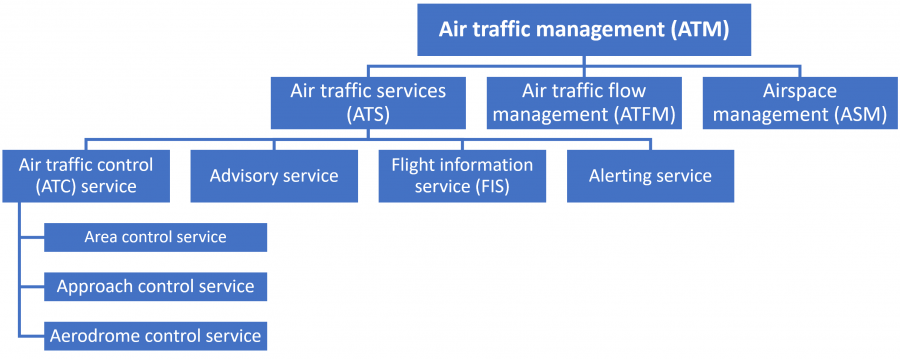
\includegraphics[width=0.8\linewidth]{900px-ATM_Chart.png}
    \caption{Structure of \gls{ATM} \cite{skybraryATM}}
    \label{fig:atm-structure}
\end{figure}

\Glspl{ATCO}, part of \gls{ATC} service, are responsible for directing aircraft safely and efficiently, managing takeoffs and landings, maintaining safe distances between aircraft en route and handling emergencies. 
Their role demands high levels of situational awareness, rapid decision-making, and the ability to manage multiple tasks under high stress conditions.
These indispensable skills, such as judgement, flexibility and the ability to handle unexpected situations, remains critical and are not easily replicated by automated systems \cite{eurocontrol2024digitalisation}.


\subsection{UAS Traffic Management (UTM)}

\Gls{UTM} is a system for safely managing \gls{UAV} operations at low altitude. 
Separate from but complementary to \gls{ATS}, it enables fucntions such as flight planning, authorisation, surveillance, and conflicht management to mitigate risks and ensure safe, efficient operations of \glspl{UAV}.
There is ongoing work to fully realize the benefits of \gls{UTM} \cite{faa_utm}.


\subsection{Challenges with Integrating UTM to ATM}

Integrating \gls{UTM} into traditional \gls{ATM}is complex but crucial for ensuring safe and efficient airspace operations, primary due to the differing nature of \gls{UAS} and manned aircrafts. 
While \gls{UTM}, designed to manage drone missions, , it must be integrated seamlessly into the existing \gls{ATM} infrastructure to prevent accidents and enhance scalability. 
Both systems must work together, as unmanned flight systems need to detect and respond to other aircraft in emergencies, and vice versa \cite{flynex2020utm_atm}.

The growing complexity of \gls{ASM}, driven by the driven by the rapid expansion of commercial aviation, \gls{UAM}, and \glspl{UAV}, has led to increased air traffic volume.
As air traffic rises, the limited capacity of \glspl{ATCO} -- who are also affected by fatigue and information overload -- becomes a major challenge \cite{Ramachandran_2025}.
Human limitations in decision-making highlight the need for AI-based solutions, such as real-time data processing and predictive analytics, to improve system performance \cite{Ramachandran_2025}.
Despite existing automation, current systems often rely on rigid frameworks that lack the flexibility needed for dynamic environments  \cite{Meier_2024}.

Additionally, \gls{UAS} have unique performance characteristics that complicate their integration into the air traffic flow, often resulting in suboptimal use of airspace capacity.
\Glspl{UAV} typically operate across both controlled and uncontrolled airspaces, and since \glspl{ATCO} only manage controlled spaces, the lack of oversight in uncontrolled airspace raises the risk of collisions or accidents. 
As a result, \gls{UTM} systems are essential for ensuring safe and efficient \gls{UAV} operations across all airspaces \cite{Zsolt_2017}, highlighting the urgent need for scalable, flexible, and automated solutions in air traffic management.


% \Gls{UAS} present additional challenges due to their unique performance characteristics, which differ from conventional aircraft. 




% However, integrating UTM into the established \gls{ATM} system, which was designed for manned aircraft, is complex and critical to ensuring safe and efficient operations \cite{flynex2020utm_atm}.

% One of the major challenges arises from the need for unmanned flight systems to detect and respond to other flying objects in emergencies, and vice versa. 
% Therefore, \gls{UTM} should be viewed as an integral part of \gls{UAS}, rather than a separate entity \cite{flynex2020utm_atm}. 
% Both systems must be as compatible as possible to ensure safe, efficient, and scalable operations in increasingly congested airspaces.

% The rapid expansion of commercial aviation, \gls{UAM}, and the widespread use of \glspl{UAV} have significantly increased the complexity of \gls{ASM} \cite{Ramachandran_2025}.
% As air traffic volume increases, the scalability of the system is constrainted by the limited capacity of \glspl{ATCO} \cite{Meier_2024}.%, who are subject to workload constraints and cognitive overload
% This problem is exacerbated by the growing fatigue and information overload experienced by ATCOs, which contribute to operational inefficiencies and safety risks \cite{Ramachandran_2025}. 
% The human limitations in reaction time and decision-making speed further underline the need for advanced automated support systems capable of enhancing the performance of \gls{ATM}.




% Integrating \gls{UAS} into air traffic flow poses a significant challenge due to their unique performance characteristics, which differ from conventional aircrafts.
% % These differences can lead to suboptimal use of airport capacity \cite{Schuchardt_2023}.
% Compounding the issue is the current shortage of \glspl{ATCO}, alongside the long training periods required to qualify new personnel, this has amplified the demand for \gls{AI}-based solutions in \gls{ATM}. 
% \gls{AI} technologies are able to solve these challenges through real-time data processing, predictive analytics, and autonomous decision-making capabilities \cite{Ramachandran_2025}. 
% While some automations already exist in some areas \cite{skybrary2025automation}, existing systems often rely on rigid rule-based frameworks and lack the flexibility and adaptability needed for dynamic environments \cite{Meier_2024}. 

% % The integration of \gls{UAV} into \gls{ATM} has led to the development of a new branch known as \gls{UTM}.
% As \glspl{UAV} often operate across both controlled and uncontrolled airspaces -- and \glspl{ATCO} are only responsible for controlled airspaces -- a key challenge arises: there is no \gls{ATC} service in uncontrolled airspaces.
% This lack of oversight increases the risk of mid-air collisions or accidents involving other \glspl{UAV}, manned aircraft, ground vehicles, or natural and artificial obstacles.
% Therefore, a dedicated system like \gls{UTM} is essential to ensure safe and efficient \gls{UAV} operations in all types of airspace \cite{Zsolt_2017}.

% The integration of \gls{UAM} and \gls{UTM} into the existing \gls{ATM} framework will not only stress current infrastructure but also require faster, more adaptive decision-making \cite{Rumba_2020} -- an area where \gls{AI} technologies can provide substantial value.




% \subsection{Current Challenges and Emerging Trends}

% The rapid expansion of commercial aviation, \gls{UAM}, and \glspl{UAV} have significantly increased the complexity of \gls{ASM} \cite{Ramachandran_2025}.
% With air traffic volume increases, the scalability of the system is limited by the finite capacity of \glspl{ATCO}, who are subject to workload constraints and cognitive overload \cite{Meier_2024}.
% Fatigue and informaion overload  have become key contributors to operational inefficiencies and potential safety risks \cite{Ramachandran_2025}. 
% Furthermore, human limitations in reaction time and decision-making speed highlight the need for intelligent, automated support systems that can enhance overall system performance.

% % Integrating \gls{UAM} into air traffic flow poses a significant challenge due to their unique performance characteristics, which differ from those of fixed-wing aircraft.
% % These differences can lead to suboptimal use of airport capacity \cite{Schuchardt_2023}.
% % Compounding the issue is the current shortage of \glspl{ATCO}, alongside the long training periods required to qualify new personnel, this has amplified the demand for \gls{AI}-based solutions in \gls{ATM}. 
% % \gls{AI} technologies are able to solve these challenges through real-time data processing, predictive analytics, and autonomous decision-making capabilities \cite{Ramachandran_2025}. 
% % While some automations already exist in some areas \cite{skybrary2025automation}, existing systems often rely on rigid rule-based frameworks and lack the flexibility and adaptability needed for dynamic environments \cite{Meier_2024}. 

% % The integration of \gls{UAV} into \gls{ATM} has led to the development of a new branch known as \gls{UTM}.
% % As \glspl{UAV} often operate across both controlled and uncontrolled airspaces -- and \glspl{ATCO} are only responsible for controlled airspaces -- a key challenge arises: there is no \gls{ATC} service in uncontrolled airspaces.
% % This lack of oversight increases the risk of mid-air collisions or accidents involving other \glspl{UAV}, manned aircraft, ground vehicles, or natural and artificial obstacles.
% % Therefore, a dedicated system like \gls{UTM} is essential to ensure safe and efficient \gls{UAV} operations in all types of airspace \cite{Zsolt_2017}.

% The integration of \gls{UAM} and \gls{UTM} into the existing \gls{ATM} framework will not only stress current infrastructure but also require faster, more adaptive decision-making \cite{Rumba_2020} -- an area where \gls{AI} technologies can provide substantial value.

% % This report explores the roles of \gls{AI} in shaping the future of \gls{ATM}, focusing particularly on its application to autonomous airliners and \gls{UAM} integration.


% \subsection{Emerging Trends}